\chapter{Technischer HintergrundWerkzeuge}

\section{erwägter Lösungsvorschlag}

\subsection{Kommunikation im Projekt Radig}
Im Projekt Radig ist keine echte Kommunikation zwischen dem Client und dem Server 
vorhanden. 

Die auf der Webseite dargestellten Werte werden vor dem senden der HTML-Seite 
im HTML-Code eingefügt indem Platzhalter im Format "`\%PORTA0"' ersetzt und so statisch auf 
der Webseite dargestellt werden. Das Manipulieren der Pins findet über ein HTML-Formular 
statt. Alle manipulierbaren Pins sind als Input vom Typ Checkbox dargestellt. Diese lassen 
sich frei manipulieren und erst beim Betätigen des "Senden"-Buttons werden die 
Informationen per POST-Event an den Server gesendet und so die Seite neu aufgerufen. Der 
Server filtert die POST Informationen aus dem HTTP-Header und manipuliert die Pins gemäß 
den Anweisungen. Beim senden des angeforderten HTML-Dokumentes werden die neuen Werte in 
den HTML-Code eingefügt, und so die neuen Werte auf der Webseite angezeigt.

Das große Problem bei dieser technisch einfachen Lösung ist, das geänderte Werte erst beim 
nächsten neu laden der Webseite angezeigt werden. Ändert sich ein Pin während die Webseite 
dargestellt wird bekommt der Nutzer dies nicht mit. Zudem wird bei jedem Manipulieren 
eines Pins die gesamte Seite neu geladen und so Unmengen an unnötigen Daten übertragen. 
Auch zum darstellen der aktuellen Werte muss die ganze Seite neu vom Server angefordert 
werden.

\subsection{Erster Ansatz}
Die Kommunikation zwischen Server und Client sollte mit Hilfe einer REST-Schnittstelle 
stattfinden, die im Hintergrund über Javascript angesprochen werden kann. 

Eine REST-Schnittstelle besteht aus einer oder mehreren virtuellen URLs. Beim Aufruf einer 
solchen URL liefert der Server kein Dokument das gespeichert ist, sondern erzeugt 
dynamisch eine Antwort mit den benötigten Informationen und sendet diese als Antwort 
zurück. Der Server kann beim Aufruf einer URL auch eine Aktion ausführen.

Vorteile der REST-Schnittstelle ist die simple Implementierung, sowohl auf dem Client mit 
JavaScript als auch auf dem Server. Die Inhalte werden mit JSON formatiert, welches einen 
technisches Standart darstellt und sich in JavaScript direkt in ein Objekt umwandeln 
lässt. Auf dem Server ist es einfach mit einem Stringformat immer gleiche JSON Strukturen 
zu erstellen und nur aktuelle Werte einzufügen. Die REST-Schnittstelle lässt sich leicht 
um weitere, neue Funktionalitäten erweitern, indem neue virtuelle URLs erstellt werden die 
vom Client ansprechbar sind.

Die Anforderungen an eine Lösung in diesem Projekt waren vor allem eine möglichst kompakte 
Schnittstelle zu schaffen die wenig Bandbreite verbraucht um eine hohe 
Übertragungsgeschwindigkeit zu ermöglichen trotz des schwachen Servers. Ein besonderes 
Augenmerk war auf die Übertragung der Messwerte zu legen, da diese nicht wie andere 
statische Informationen nur einmalig übertragen werden sondern kontinuierlich erneuert 
werden müssen. Die Schnittstelle sollte gut skalierbar sein. Würde später ein Port für
eine andere Aufgabe zu verwendet werden muss dieser Port ohne Aufwand aus der 
REST-Schnittstelle ausgeschlossen werden können, damit er von außen nicht manipulierbar 
ist und so interne Abläufe auf der Platine nicht gestört werden.

Nach den Anforderungen muss die Schnittstelle folgende Aufgaben ermöglichen:
\begin{itemize}
\item Abfragen der aktuellen Werte aller verwendbaren Pins
\item Abfragen der Konfiguration eines Pins (Eingang oder Ausgang)
\item Abfragen von Allgemeinen Informationen des Boards (IP, Standart-IP, Mac-Adresse,
	Serverversion)
\item Manipulieren aller als Ausgänge geschaltener Pins
\item Manipulieren der Konfiguration eines Pins (als Eingang oder Ausgang setzen)
\item Manipulieren von Servereinstellungen (z.B. IP-Adresse);
\end{itemize}

%\begin{itemize}
%	\item Aufbau als REST-Schnittstelle
%	\begin{itemize}
%		\item Simpel implementierbar
%		\item Technischer Standart
%		\item Fertige Mechaniken in JavaScript
%		\item Leicht erweiterbar um neue Funktionalitäten
%	\end{itemize}
%	\item Anforderungen an eine Lösung:
%	\begin{itemize}
%		\item Möglichst kompakt, wenig Bandbreite soll verbraucht werden
%		\item Messwerte müssen besonders effizient übertragen werden
%		\item Skalierbar - Egal ob ein oder 20 Ports verwendet werden
%		\item Neben Abfragen der Messwerte auch manipulieren der IP, des DDR und der 
%			  Ausgänge
%		\item JSON-Encodiert, direkt in JavaScript Objekt überführbar
%	\end{itemize}
%\end{itemize}

%-----------------------------------------------------------------------------------------
\subsection{Polling oder Pushing}
Die aktuellen Werte der Pins müssen bei jeder Änderung vom Server zum Client übertragen 
werden, damit diese auf der Webseite immer korrekt dargestellt werden. Hierfür stehen zwei 
verschiedene Konzepte zur Verfügung wie die Übertragung der Daten initialisiert werden.

\subsubsection{Polling}
Bei Polling werden vom Client kontinuierlich die Werte erneut angefordert, indem dieser 
die entsprechende virtuell URL des Servers aufruft. Dies führt dazu, dass viele unnötige 
Date übertragen werden, da sich eventuell nicht bei jedem erneuten anfordern der Werte 
diese auch tatsächlich verändert haben und so die gleichen Datensätze oft mehrmals 
angefordert werden.

Im vergleich zu der Radig-Lösung bietet Polling den Vorteil das die Werte kontinuierlich 
nach geladen und so immer korrekt dargestellt werden während die Webseite dargestellt 
wird. Auch das gesendete Datenvolumen wird dahingehend minimiert, das nur die Nutzdaten 
übertragen werden und nicht der gesamte HTML-Code der Webseite. Polling ist technisch sehr 
einfach zu realisieren, da die Abfrage der Daten einfach zyklisch wiederholt werden.

\subsubsection{Pushing}
Bei Pushing wird im Gegensatz zu Polling der Daten nicht vom Client initialisiert sondern 
vom Server. Der Server weiß wann sich die Werte geändert haben und kann dem Client bei 
jeder Änderung gezielt die neuen Daten Übermitteln. Das Übertragen der Daten könnte z.B. 
durch einen Interrupt ausgelöst werden.

Im direkten vergleich zu Polling bietet Pushing verschiedene Vorteile. So wird nicht nur 
das Volumen der übertragenen Daten reduziert indem keine unnötigen Abfragen stattfinden,
sondern die neuen Werte gelangen auch genau dann zum Client wenn die Änderung tatsächlich 
stattgefunden hat, was dazu führt das die Webseite schneller auf Änderungen reagiert.

Die technische Umsetzung von Pushing ist mit diversen Problemen verbunden. Die typische 
Verbindungsaufbaurichtung ist bei Webanwendungen und Webseiten immer vom Client zum 
Server. Anders als bei Polling müssen bei Pushing Daten vom Server zum Client gelangen. 
Hierfür muss eine Verbindung vom Server zum Client aufgebaut werden. Dies ist technisch 
aber nicht möglich, da der Browser bzw. JavaScript keine Möglichkeit haben einen Port des 
Clientsystems zu öffnen und auf eingehende Verbindungen des Servers zu antworten. 

Das Problem lässt sich durch die Benutzung von HTML5 Server-Sent Events umgehen. Hierbei 
frägt der Client eine virtuelle URL des Servers ab, ähnlich einer REST-Schnittstelle. Der 
Server überträgt jedoch nicht sofort Daten, sondern schreibt erst bei einem Event (z.B. 
die Änderung eines Pins) in den geöffneten Stream und pusht so die Daten zum Client. 
Dieser überwacht den Stream mit Hilfe von JavaScript un empfängt so die neuen Werte und 
kann sie auf der Webseite anzeigen.

Dieses System ist auf dem Pollin Net-IO Board aber nur schwer umzusetzen da mehrere 
Verbindungen verwaltet werden müssen. So ist immer mindestens eine Server-Sent Event 
Verbindung offen, parallel könnte aber ein Client andere Daten vom Server anfordern. Für 
das Verwalten mehrerer Verbindungen sind aber viele Resourcen nötig, da für jede 
Verbindung auch Daten im RAM hinterlegt werden müssen. Außerdem st in vielen Situationen 
ein simples Multitasking nötig, das so auf einem ATmega CPU nicht vorhanden ist. Das Radig 
Projekt setzt aus diesen Gründen auf HTTP 1.0 bei dem für jede Anfrage eine Verbindung 
geöffnet und nach erfolgreichem Übertragen der Daten wieder geschlossen wird. So ist auch 
die Kommunikation mit mehreren Clients problemlos möglich.

Um HTML5 Server-Sent Events auf dem Pollin Net-IO Board zu implementieren würde es als 
einen tendenziell größeren CPU erfordern mit dem auch Multitasking möglich ist sowohl auch 
eine grundlegende Umgestaltung des Radig-Projektes um mehrere HTTP Verbindungen parallel 
zu ermöglichen.

\subsubsection{Entscheidung}
Da die technische Umsetzung vom Pushing nur schwer möglich ist werden wir auf Polling 
setzen.

TODO: Hier noch Argumentation mit Übertragungszeit und Screenshot aus Chrome Network Log


%\begin{itemize}
%	\item Daten können entweder per Polling vom Client (Webseite abgefragt werden) oder
%		  vom Server bei einem Event (Änderung eines Eingangs) per Push geschickt werden	  
%	\item Pro/Contra Push
%	\begin{itemize}
%		\item Pro: Daten werden nur übertragen wenn es wirklich nötig ist, kein unnötiger 
%			  Datenverkehr
%		\item Pro: Leistung bleibt auch mit mehreren Clients eher konstant 
%			  (Genau Begründung ausarbeiten!)
%		\item Pro: Board wird entlastet, kein DOS, mehrere Clients können Webseite 
%		      trotzdem problemlos aufbauen 
%	\end{itemize}
%	\item Pro/Contra Polling
%	\begin{itemize}
%		\item Pro: Leichter zu implementieren - normale Dateiabfrage
%		\item Contra: Es werden viele unnötige Daten übertragen
%		\item Contra: Leistung nimmt mit steigender Anzahl von Clients ab
%		\item Pro: Im Prinzip nicht langsamer als Push: Limitierende Komponente ist die 
%			  Übertragungszeit! (Hier Bild von Chrome Netzwerkvehrkehr) 
%	\end{itemize}
%	
%	\item Push bessere Lösung
%	\item Umsetzung aber nicht möglich
%	\item Server kann keine Verbindung zu Client aufbauen
%	\begin{itemize}
%		\item Javascript kann keinen Serverport öffnen
%		\item Client hat keine öffentliche IP
%	\end{itemize}
%	\item Technische Lösung: HTML 5 Server Sent Events
%	\begin{itemize}
%		\item Technischer Standart, Eingeführt mit HTML 5
%		\item Client ruft virtuelle URL auf, ähnlich REST
%		\item So wird ein Stream geöffnet
%		\item Bei einem Event schreibt der Server die Informationen in den Stream
%		\item Client benutzt Javascript API um die jeweiligen Informationen zu lesen
%	\end{itemize}
%	\item Mit ATmega CPU und Radig Projrkt als Vorlage nicht lösbar
%	\begin{itemize}
%		\item Radig kann nur eine Verbindung handeln. Aufbau - Übertragung - Abbau für 
%			  jede Datei
%		\item HTTP 1.0
%		\item Aufruf einer HTML5 Server Sent Event URL würde dazu führen das der Server 
%			  blockiert ist
%		\item Gesamte Struktur auf nur eine Verbindung ausgelegt
%		\item Bei Umschreiben (sehr tiefer Eingriff!) stößt die CPU schnell an Grenzen
%		\item Multitasking nötig, Stack für jede Verbindung führt zu RAM Problemen
%		\item Sprengt vermutlich zeitlichen Rahmen
%	\end{itemize}
%	\item Daraus resutltiert die Verwendung von Polling
%	\item Da Polling nicht langsamer ist, gibt es keine Nachteile bei Frequenzen von ca. 
%		  200ms (auch bei zB. 3 Clients)
%\end{itemize}

%-----------------------------------------------------------------------------------------
\subsection{Aufbau der REST-Schnittstelle}

\begin{itemize}
	\item 6 URLS
	\item ..........Hier Zitat aus Präsentation, aber noch anpassen!
\end{itemize}
	
%-----------------------------------------------------------------------------------------
\subsection{Implementierung der REST-Schnitstelle auf dem Server}

Für die Restschnittstelle wurde Weitestgehend der Bestehende Quellcode von Radig
verwendet. Zum auslesen ob ein Pin gesetzt ist sind Platzhalter vorgesehen.
Das Schema für so einen Platzhalter ist \textrm{\%PINXY} und setzt sich zusammen aus dem
Aufruf \textrm{\%PIN}, dem anzusprechendem Port X = [A,C oder D] und dem Pin Y = [0-7] (z.B.
\textrm{\%PINC1 } ). Mit diesem Platzhalter kann der direkte Pin Ausgelesen
(Hier Port C und Pin 1) und an eine beliebige Stelle im Quellcode platziert werden. Neu
hinzugekommen ist das Ausgeben der Information ob der Konkrete Pin über das
DDRegister als Ein- oder Ausgang definiert ist. Das Schema ist für diesen
Platzhalter ist \textrm{\%DDRXY} und setzt sich zusammen aus dem Aufruf \textrm{\%DDR}, dem
anzusprechendem Port X = [A,C oder D] und dem Pin Y = [0-7] (z.B.
\textrm{\%DDRD1} ). \\
\\
Damit das System für uns möglichst flexibel Arbeitet, haben wir uns dafür
entschieden, diese Dynamischen Angaben in eine Separate Datei auszulagern und
über die REST Schnittstelle abzufragen. Konkreter liegt in dem /Rest
Verzeichnis eine \textrm{values} Datei die die Platzhalter enthält. Zusätzlich
gibt es noch eine \textrm{info} und \textrm{pininfo} Datei, die statische
Informationen zu den Pins und Ports Enthält. \\
\\
Das setzen der Ausgänge wird über einen HTTP-Post Aufruf getätigt. So können die
Pins des entsprechenden Ports gesetzt oder umgeschaltet werden. Die
Informationen, die zum setzen eines Ports benötigt werden setzen sich zusammen
aus einem \textrm{SET} Befehl und dem Aufruf PORTXYZ zum setzen oder dem
\textrm{SET} Befehl und dem Aufruf OUTXYZ. X steht für den anzusprechendem Port
X = [A,C oder D]. Y und Z Stehen für die Einstellung der Pins in hexadezimaler
Schreibweise (00-FF) Abschließend muss das Ende der Schaltanweisung mit
\textrm{SUB} gekennzeichnet werden, da der Webserver auf diese Steuerzeichen
prüft. Ein Beispiel Post zum setzen der Pins C0-C3 auf Ein, der Pins C4-C7 auf
Aus, dem umschalten der Pins D0-D3 als Ausgang und der Pins D4-D7 als Eingang
sieht folgendermaßen aus:
\\

\framebox{SET=PORTC0F\&SET=OUTD0F\&SUB=Senden} 
%\begin{itemize}
%	\item Benutzung der Struktur von Radig
%	\item Die Eingägne werden durch Platzhalter (z.B. \%PortC1 ) angegeben. Beim
%			übertragen des Dokuments werden die Platzhalter ersetzt durch passende Werte
%	\item in /rest liegen Dateien values (mit Platzhaltern), pininfo und info
	% (jeweils als
%	      statisches Dokument)
%	\item Dateien können von ausßen normal aufgerufen werden und werden ggfs. mit
	% realen
%	      Informationen aufgefüllt
%	\item Vorteil: Test außerhalb der Platine möglich, da Werte als String
	% gekennzeichnet
%	      sind in JSON, Pins haben dann den Wert \%PortXY anstatt 0 oder 1
%	\item TODO: Wie werden die set URLs implementiert?
%	\item Die Ausgänge werden über die Post übertragung gesetzt.
%\end{itemize}

%-----------------------------------------------------------------------------------------
\subsection{Implementierung der REST-Schnitstelle auf dem Client}

\begin{itemize}
	\item Aufruf der URLs im Hintergrund mit Ajax
	\item info und pininfo werden zu Beginn einmalig aufgerufen (synchron um zu 
	      gewährleisten das die Daten zur Verfügung stehen für andere Initialisierungen)
	\item values wird mit setTimeout(...) zyklisch assynchron aufgerufen
	\item synchrones aufrufen von values führt dazu, das sich die Webseite aufhängt, da
	      der (Single-)JavaScript Thread mit dem laden der Daten beschäftigt ist und nicht
	      für andere Aufgaben zur Verfügung steht. Bei einem assynchronen Aufruf werden 
	      die Daten von einem anderen Thread im Hintergrund geladen
	\item JSON-Text wird mit JSON.parse(...) in ein Objekt transformiert
	\item Informationen werden über entsprechende getter zur Verfügung gestellt
	\item Funktion onValueChanged wird jedes mal aufgerufen wenn neue Daten zur 
	      Verfügung stehen
	\item onError wird aufgerufen wenn ein Fehler in der Kommunikation aufgetreten ist
	\item Über setter werden die entsprechenden URLs assynchron aufgerufen und so die 
	      Daten an den Server übermittelt
\end{itemize}

\section{Tools und Werkzeuge}

\subsection{Das Atmel Studio}

\subsubsection{DeviceProgramming}

Gerät Auswählen
Contoller Auswählen
Spannung und Signatur
Fuse Bits
Hexfile Flashen

\begin{figure}[h]
\centering
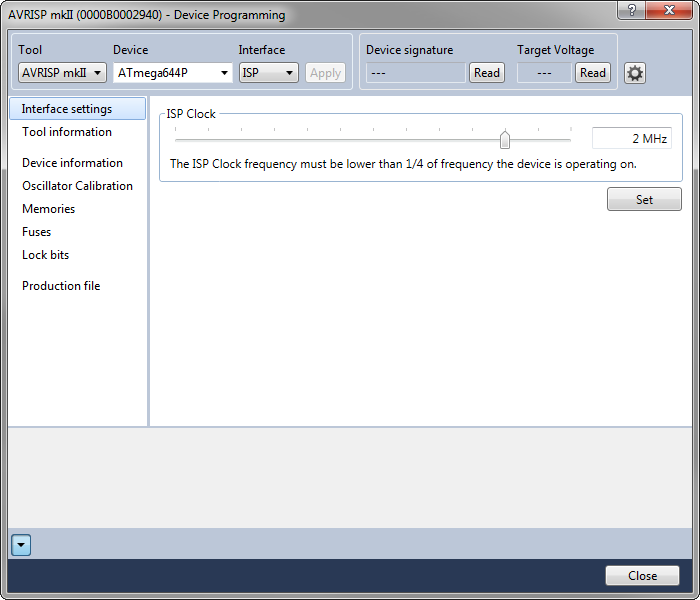
\includegraphics[width=13cm]{content/pictures/Anleitung/neuerProzessor/AnleitungNeuerProzessor1.png}
\caption{DeviceProgramming}
\label{fig:B3}
\end{figure}

\subsubsection{Projekt Einstellungen}

Taktfrequenz
Programmer
Empfolene Tool Settings

\subsection{AVRDUDE}

\subsection{HTML Header Compiler}

\section{Prozessorgrößen}

\section{System Architektur}

\begin{itemize}
\item Was soll hier rein??
\end{itemize}

